\part{Implementation}

\setcounter{chapter}{0}

\chapter{Works Done}

\section{What we implemented}

During two and a half months of this project, we implemented both models which were described in the article. As a reminder, these two models are a simple random and a model concerning pheromones. We also implemented the Random Waypoint model on the demand of our clients. In this section, we will explain the development work that we have provided and the different choices.


\subsection{Random model} 

To implement this model, we needed four classes.\\
The first class, which is called \textit{Main.java}, allows as its name indicates it, launching the program. It is in this class that we define the size of the window, the matrix which will serve to simulate the scan of a zone (all the nodes will have the same matrix), and the instanciation of the various objects coming of JBotSim library. We have for example, an object named \textit{topo} which is a topology. This object is the basis for our simulator. It is to this topology that we are going to be able to add mobile nodes (here planes).\\

We also instantiated a Jtopology's object type. We will explain this choice during the presentation of entities.\\

The second class of our architecture is called \textit{MovingNode}. It is in this class that will be handled the movement of the various nodes. That's why this class inherits from the class \textit{Node} and implement the interface \textit{ClockListesner}, both coming from the JBotSim librairies. It inherits from the class \textit{Node} because planes will be represented by mobile node, so we need the characteristics of that class. Moreover, It implements the interface \textit{ClockListener} because we need that our nodes move all the seconds, so we need a top of clock to realize it. We will have a listener for time , as well as a method \textit{onClock} which will be called to every top of horloge.\\

This class contains a constructor by default, allowing to instantiate and to initialize the different variable, and to associate images with the mobile nodes (call of the method \textit{setProperty}). The random model gets characteristic to have no communication between the different nodes. To realize it, we pass an argument of \-1 in the method \textit{setCommunicationRange}.\\

As indicated in the article, the nodes of the random model change actions every seconds in functions of the last undertaken action. As a reminder, here is the table of action for the random model:\\

\begin{figure}[h]
\center
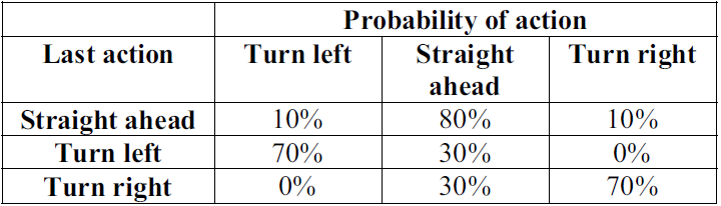
\includegraphics[width=15cm]{../images/table_random.png}
\caption{UAV random action table\cite{UAV}}
\end{figure}

In our implementation, we have a variable \textit{lastdirection} allowing to know the last action which was made. We associated figures with the last actions. If the last direction was the left, then the variable \textit {lastdirection} takes the value 1, if it was straight, then we associate the value 2, and if it was to the right, we associate the value 3.\\

To respect as much as possible the reality, we had to modify the management of the edges of the window. Indeed, originally in JBotSim, nodes can pass from an edge to the other one. For example, if they reached the left edge, they went to the right of the window, what is not possible in the real life. We blocked this problem by rectifying the position of the node, and by changing its angle of direction.\\

Each time a node scans a zone, it looks in the matrix if this position was already scanned (0 if the zone was never scanned, 1 otherwise). If it is, then it makes nothing, otherwise it puts the value to 1.\\

The third class of our architecture is called \textit{Jtopology\_Random}. It inherits from JTopology and is going to draw the scans footprint on the map. This class JTopology inherits from JPanel, and is situated in fact between a JViewer and a Topology.

The last class 
\subsection{Random Waypoint Model}

This model is very similar to the previous. The only difference is their way to move.\\
In this model, the node choose one point randomly and move to it.\\
So the only modification compared to the previous model is the class \textit{MovingNode} and more precisely the method \textit{onClock}.\\
In this method, we choose a random point and we move the node until it. To do this, we change the direction of the node to the direction of the point chosen. When the node arrive at this point, we choose an other random point and so on.\\
In this model, we don't manage the edge of the window because all destination point are chosen on the window and so none UAV can go out the window.

\subsection{Pheromone model}

Concerning the architecture, the implementation of the model of pheromones is very similar. We find practically 3 even classy. Only the class \textit{MovingNode} is really going to be different because the movements of nodes are going to depend on a lot of parameter. First of all, this class implements a new interface which is \textit{MessageListener}. Indeed, in this model, nodes have to sent data each others (in this particular case their respective map).\\

The method which is going to change compared with the random model is the method \textit{onClock}. Indeed, it is here that we are going to apply rules as described on the following image:

\newpage

\begin{figure}[!h]
\center
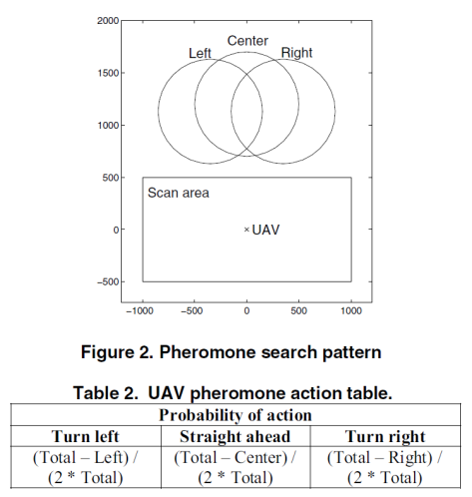
\includegraphics{../images/pheromon_model.png}
\caption{Pheromone search pattern\cite{UAV}}
\end{figure}

\begin{figure}[!h]
\center
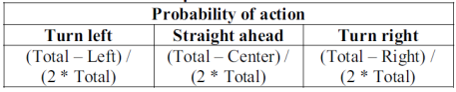
\includegraphics{../images/pheromone_table.png}
\caption{UAV pheromone action table\cite{UAV}}
\end{figure}

We handled all the cases described in the article, meaning node looks at the values of pheromones in its left diagonal, in front of him and in its right diagonal.

\newpage

\begin{figure}[!h]
\center
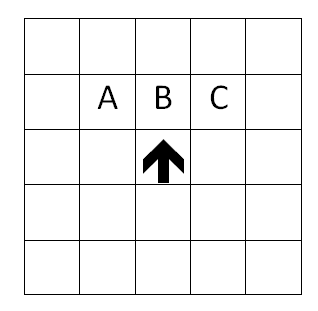
\includegraphics[width=5cm]{../images/grille_case_1.png}
\caption{\label{case1}case 1}
\end{figure}

\begin{figure}[!h]
\center
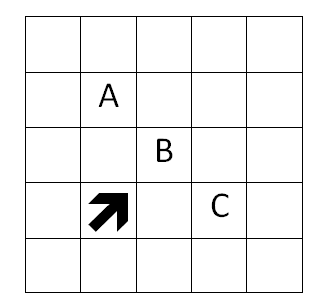
\includegraphics[width=5cm]{../images/grille_case_2.png}
\caption{\label{case2}case 2}
\end{figure}

These both cases \ref{case1} and \ref{case2} show how a node scan the map.

\begin{itemize}
\item the area A represents the left diagonal of the node.
\item the area B represents the front of the node.
\item the area C represents the right diagonal of the node.
\end{itemize}

We handle the communication between each node with the \textit{MessageListener} and the method \textit{onMessage}. This method is called when a node do the method \textit{send}. We have no destination in the method \textit{send} to broadcast the message. We send message all ten top of clock to respect the conditions of the scenario of the article.

\newpage

\section{Difficulties Encountered \& Solutions}

The bigger difficulty encountered has been reading a lot of articles, like references of our main article. Indeed, they included many pages and the reading of them in english took us a lot of time. We had to update each of them on internet in order to learn the evolution of the differents models, the technologies used, etc.\\

Concerning the implementation, we did not meet many difficulties. The only big problem is the display of the scanned zones. On the advice of Mister Casteigts, we should create a class inheriting from JTopology and redefine the \textit{paint} method. Indeed, the display refreshment of the scanned zones is a problem because we lost scanned zones previously. We created an ArrayList to save area scanned to redraw them in every times.\\

We have also an other trouble with the displaying. The UAV are drawn under the pheromones.
